\documentclass{article}
\usepackage[T1]{fontenc}
\usepackage[utf8]{inputenc}
\usepackage{amsmath}
\usepackage[brazil]{babel}
\usepackage{graphicx}
\usepackage{listings}
\lstset{
    basicstyle=\ttfamily
}


\author{Tiago Royer}
\title{Analisador de Dendogramas}

\begin{document}

\maketitle

\section{Introdução}

Dendogramas é uma forma de representação de dados em árvores,
em que entradas de dados similares são agrupadas sob o mesmo ramo.
Dendogramas podem ser usados para induzir classificadores:
basta cortar a árvore em algum ponto,
e considerar que os dados que ficaram no mesmo ramo pertencem à mesma classe.

O objetivo deste trabalho era implementar um analisador de dendogramas;
dado um conjunto de dados,
o programa deve construir um dendograma
e encontrar um ponto ótimo de corte na árvore,
respeitados um limite mínimo e máximo para o número de classes.

Meu código está disponível em \verb"https://github.com/royertiago/INE5443".

\section{Interface com o usuário}

Construí o analisador de dendogramas usando, como base,
as classes já implementadas para os trabalhos 1 e 2
($k\mathit{NN}$ e Mahalanobis; IBL).
Em particular, extendi o formato do conjunto de dados
para nomear as entradas de dados;
estes nomes são usados na visualização do dendograma.
Usarei como exemplo o conjunto de dados \verb"datasets/mtcars.data".

Após a compilação (invocando \verb"make"),
o programa pode ser invocado com \verb"./dendogram".
Este programa lerá um conjunto de dados da entrada padrão,
construirá um dendograma,
e o exibirá na tela.
Pressione qualquer tecla para sair.
Assim como todos os outros programas do repositório,
a maior parte da funcionalidade do programa está ``escondida'' 
nas opções de linha de comando;
para uma listagem completa das opções,
execute \verb"./dendogram --help".

Chamar o programa sem opções produz a imagem exibida na figura \ref{dendogram-simple}.

\begin{figure}[h]
    \makebox[\textwidth][c]{
        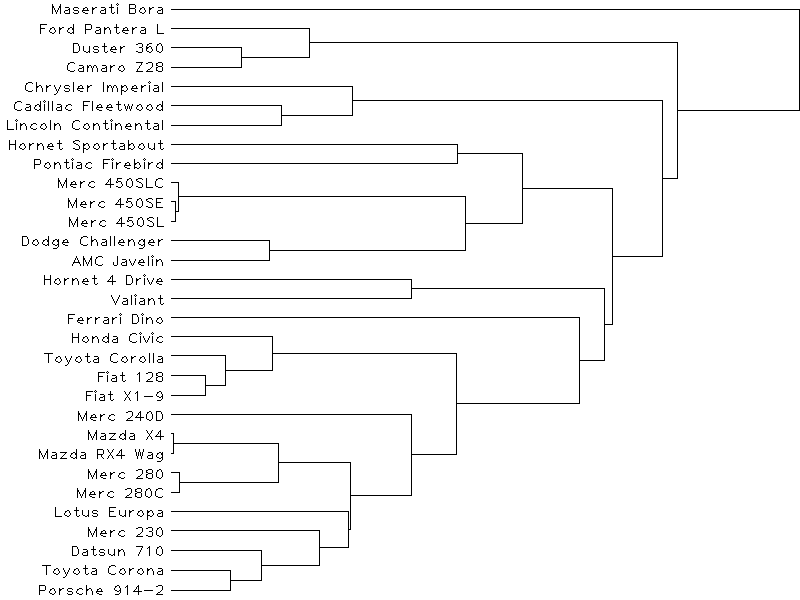
\includegraphics[scale=0.5]{dendogram-simple.png}
    }
    \caption[]{
        Dendograma gerado para o conjunto de dados \texttt{mtcars.data},
        usando distância de conexão simples.
        Comando:

        \lstinline"./dendogram < datasets/mtcars.data"
    }
    \label{dendogram-simple}
\end{figure}

Foram implementadas três interpretações diferentes
para a distância de conexão entre dois conjuntos:
simples, completa e média.
O algoritmo pode ser selecionado usando as opções
\verb"--simple", \verb"--full" ou \verb"--mean" na linha de comando.
O padrão é \verb"--simple",
que é o que aparece na figura \ref{dendogram-simple}.

Por padrão, o programa não faz alterações no conjunto de dados.
A opção \verb"--normalize" normaliza todas as dimensões para o intervalo $[0, 1]$.
A opção \verb"--standardize" reescreve cada dimensão em termos de
quantidades de desvios-padrão distante da média.

A imagem \ref{dendogram-mean} foi gerada usando \verb"--mean" e \verb"--standardize".

\begin{figure}[h]
    \makebox[\textwidth][c]{
        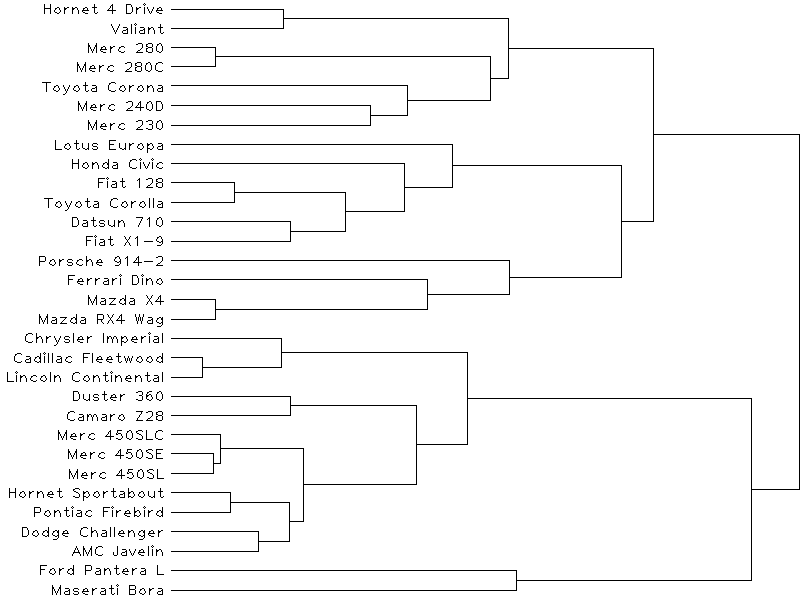
\includegraphics[scale=0.5]{dendogram-mean.png}
    }
    \caption[]{
        Dendograma do conjunto de dados \texttt{mtcars.data}
        usando distância de conexão média e padronização.
        Comando:

        \lstinline"./dendogram < dataset/mtcars.data --mean --standardize"
    }
    \label{dendogram-mean}
\end{figure}

\subsection{Análise do dendograma}

Por padrão, o programa apenas gera o dendograma.
As opções \verb"--min-class" e \verb"--max-class" habilitam a análise do dendograma;
o programa encontrará um ``ponto ótimo de corte''
e imprimirá, na saída padrão,
o mesmo conjunto de dados,
mas agora classificado de acordo com o corte.

A opção \verb"--showsplit" mostra uma linha vermelha
onde o algoritmo escolheu fazer o corte;
a opção \verb"--showlimits" exibe linhas cinzas representando as posições de
\verb"min-class" e \verb"max-class".

Importante notar que as opções \verb"--normalize" e \verb"--standardize"
alteram o conjunto de dados.

A figura \ref{dendogram-full} foi gerada usando padronização;
limitando a quantidade de classes ao intervalo $[3, 10]$,
o algoritmo decidiu criar $5$.

\begin{figure}[h]
    \makebox[\textwidth][c]{
        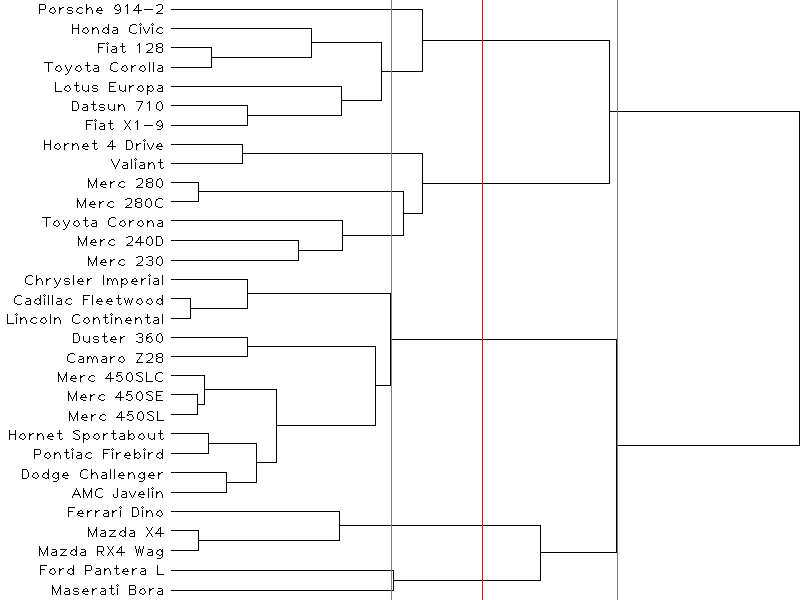
\includegraphics[scale=0.5]{dendogram-full.png}
    }
    \caption[]{
        Dendograma do conjunto de dados \texttt{mtcars.data}
        usando distância de conexão máxima e padronização.
        O algoritmo escolheu criar $5$ classes;
        o corte é representado pela linha vermelha.
        Comando:

        \texttt{./dendogram < datasets/mtcars.data -{}-standardize -{}-full 
        -{}-min-class 3 -{}-max-class 10 -{}-showsplit -{}-showlimits}
    }
    \label{dendogram-full}
\end{figure}

\section{Algoritmos implementados}

Três algoritmos principais precisavam ser implementados:
criação do dendograma, visualização e análise.

\subsection{Criação do dendograma}

A implementação direta
(manter uma lista de nodos e, a cada ``rodada'',
encontrar o par mais próximo)
possui complexidade $O(n^5)$.
(São $n$ rodadas, cada rodada com $O(n^2)$ buscas em pares,
cada busca num par custando $O(n^2)$ cálculos de distância.)

No núcleo do algoritmo,
a operação de recálculo das distâncias de conexão entre um par de nodos 
pode ser acelerada se nós armazenarmos as distâncias entre os nodos filhos.
Baseando-me nessa observação,
consegui reduzir a complexidade para $O(n^3)$.

O algoritmo, implementado em \verb"pr/dendogram.cpp",
recebe como parâmetro
o conjunto de dados e as funções $d$ e $u$.

A função $d$ (nomeada \verb"distance" no código fonte)
computa a distância de conexão entre dois nodos do dendograma.
Por exemplo, para distância de conexão mínima,
esta função retorna a menor distância entre quaisquer dois elementos,
um em cada uma das subárvores que lhe são fornecidas.

Espera-se que esta função possua complexidade proporcional
ao produto dos tamanhos das subárvores
(complexidade quadrática).
No algoritmo ingênuo, esta função é chamada $O(n^3)$ vezes
dentro do laço principal
($O(n^2)$ por iteração),
resultando na complexidade quíntica.
Idealmente, $d$ deveria ser uma operação constante
para ser chamada tantas vezes assim dentro do laço.

É aí que entra $u$ (nomeada \verb"update" no código fonte).
Esta é uma função de quatro variáveis,
$a, b, d_1, d_2$,
aplicável somente se $b$ não for um nodo folha.
$u(a, b, d_1, d_2)$ deve retornar, exatamente, $d(a, b)$;
mas $u$ pode assumir que $d(a, b.\textrm{left}) = d_1$
e que $d(a, b.\textrm{right}) = d_2$.
(Chamei-a de \verb"update" porque ela calcula a distância entre dois nodos
baseando-se na distância antiga, entre um dos nodos e os filhos do outro nodo.)

Por exemplo,
$u$ para distância de conexão mínima é
\begin{equation*}
    u( a, b, d_1, d_2 ) = \min(d_1, d_2).
\end{equation*}

O fato de $u$ ser computável em tempo $O(1)$
garante o aceleramento do algoritmo.

\subsection{Visualização}

Graças à funcionalidade de criação de submatrizes do OpenCV,
a implementação da visualização foi relativamente simples.

Caso o nodo atual não seja folha,
o algoritmo cria duas subregiões na região que lhe foi dada,
com dimensões proporcionais aos tamanhos dos nodos filhos
e às distâncias de conexão destes nodos.
Então, basta chamar a função que desenha o dendograma recursivamente
e conectar os dois ramos ao final.

Desta forma,
ficou bastante simples implementar a característica de que
a ``altura'' da ligação é proporcional à distância de conexão
entre as duas subárvores.

\subsection{Analisador}

Para impor algum critério de otimalidade no local de corte,
decidi fazer uma analogia entre a distância de conexão
e o esforço de ``juntar'' dois nós.

Considere, por exemplo, os quatro modelos
\verb"Mazda X4", \verb"Mazda X4 Wag", \verb"Merc 280" e \verb"Merc 280 C",
as 5ª a 8ª folhas de baixo para cima na figura \ref{dendogram-simple}.
A distância de conexão entre \verb"Merc 280 C" e \verb"Merc 280"
é maior do que a entre \verb"Mazda X4" e \verb"Mazda X4 Wag";
intuitivamente,
o ``esforço'' para unir os dois últimos
é maior do que o esforço para unir os dois primeiros.
Entretanto, o esforço para unir estes quatro nós juntos
é muito maior do que as duas outras uniões;
portanto, aquele parece ser um bom ponto de corte
(assumindo que estivéssemos falando apenas daqueles quatro nodos).

É exatamente esta a característica que meu analisador busca maximizar.
Dada uma lista
\begin{equation*}
    c_{\textit{minClass}}, c_{\textit{minClass+1}}, \dots, c_{\textit{maxClass}}
\end{equation*}
de cortes ``por alto''
(isto é, $c_i$ separou os $i$ nodos com maior distância de ligação),
o algoritmo busca um $c_k$ tal que
o esforço de juntar os dois nodos mais próximos de $c_{k+1}$,
para ficar igual a $c_k$,
seja máxima.

A noção de ``esforço de juntar dois nodos'' é entendida como
\begin{equation*}
    \textrm{nmax}(c_k) - \textrm{nmax}(c_{k+1}),
\end{equation*}
em que $\textrm{nmax}(c_i)$ é a maior distância de conexão dentro do corte $c_i$.

O algoritmo simplesmente itera sobre todos os cortes $c_i$,
$\textit{minClass} \leq i \leq \textit{maxClass}$,
calculando a diferença de esforço conforme a equação anterior,
e retorna o corte que der valor máximo.

No desenho do dendograma,
este critério de otimalidade produzirá uma linha vermelha
que estará à maior distância mínima até qualquer ponto de junção de qualquer nó.

\end{document}
